%!TEX root = ../MasterThesis.tex

\section{The Semantic Web}
\label{sec:semantic_web}

\subsection{Vision}
\label{sec:semantic_vision}

make information on the Web accessible to machines \\
- allows integration of information across web sites \\
- is also known as the ``Web of Data'' \\
\\
design principles: \\
1. make structured and semi-structured data available in standardized formats \\
2. make individual data elements and their relationships accessible on the Web \\
3. describe the intended semantics of the data in a machine readable format \\
\\
HTML is just for human consumption and a lot of the structures and semantics of the
underlying databases is lost in the transformation process \\
- use labeled graphs as data model for objects and their relationships (objects == nodes,
edges == relationships between them) \\
- formalize the syntax of the graph in RDF (Resource Description Framework) \\
- use URIs to identify individual data items and relations \\
- use ontologies to represent semantics of the data items (either lightweight RDF schema definitions
or Web Ontology Language are used for that) \\
\\
RDFS and OWL are meta-description languages allowing to define new domain-specific knowledge representations \\
they rely on the basic principles of the Web: supporting distributed, decentralized architectures \\
\\
some new initiatives for standardizing semantics: schema.org and linkeddata.org \\
initially it was tried to solve the integration issues with XML, but as it is syntactically more machine-
readable it lacks the semantic of the data \\
- as of this RDF is the basic language of the Semantic Web and describes meta-data as well as content \\
\\
an ontology formally describe a domain based on terms and their relationships (terms == classes of objects) \\
hierarchies are supported (even multiple inheritance between objects) \\
ontologies also include: \\
- properties \\
- value restrictions \\
- disjointness statements \\
- specifications of logical relationships \\
goal is to provide a shared understanding of a domain \\
can help with the necessity to overcome differences in terminology \\
a mapping for different wordings in an ontology or between ontologies is possible \\
they can also be useful for generalization or specialization of Web search results \\
\\
ontologies help with reasoning of objects, they can uncover unexpected relationships and
inconsistencies as well as - by utilizing intelligent web agents - make decisions and select course of actions
(e.g. ``if-then-conclusions'' aka Horn logic) \\
agents can also be used for ``validation of proof'' of statements of another agent or machine \\
\\
Semantic Web is a layered approach \ldots

\begin{figure}[H]
	\centering
		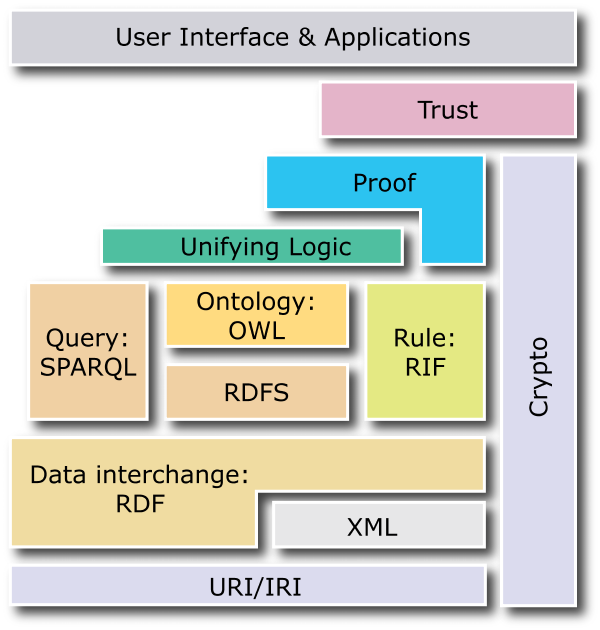
\includegraphics[height=2.5in]{images/semantic_web_layers.png}
	\caption{The Semantic Web Model \citep{W3C2013}}
\label{fig:images_semweb_model}
\end{figure}

% section semantic_vision (end)

\subsection{Resource Description Language}
\label{sec:semantic_rdl}

what is needed to exchange information? \\
1. syntax: how to serialize the data? \\
2. data model: how to structure and organize the data? \\
3. semantics: how to interpret the data? \\
\\
HTML is made for rendering information on screen and for human consumption \\
RDF brings a flexible data model to the Web: \\
- basic building block is a \textbf{triple} of \textit{entity - attribute - value}
also known as statement (could also be expressed as \textit{subject - predicate - object}) \\
RDFS describes the vocabulary that is available \\
\\
so: \\
1. syntax: Turtle, RDFa, RDF-XML or JSON-LD \\
2. data model: RDF \\
3. semantics: RDFS \\
\\
foundational elements are: \\
- resources (aka just a ``thing'' of interest identified by an URI or URL depending on its accessibility) \\
- properties (specify the relations between resources, also identified by URIs) \\
- statements (assign a value to a `resource-property' relation, value could be another resource or a literal) \\
- graphs (RDF is a graph-centered data model, could be distributed, Web of Data / Linked Data approaches) \\
\\
linked data principles: \\
- use URIs as name for things \\
- use HTTP URLs so ppl. can look up those things on the Web \\
- if they do so, provide useful information (HTML and/or RDF, content and/or meta data) \\
- include links to other URLs so they can discover more/related things \\
\\
named graph: \\
- can be used to point to specific statements or (sub-)graphs \\
- alternative: reification via an auxiliary object \\
\\
Turtle: Terse RDF triple language \\
- \textless subject incl. URI\textgreater \textless predicate incl. URI\textgreater \textless object incl. URI\textgreater . \\
- literals will be expressed as ``value''\^{}\^{}\textless XML schema data type\textgreater and supports \textit{string, integer, decimal, dates, \ldots} \\
- URIs can be prefixed: @prefix: \textless URI\textgreater \\
- repetition: `;' repeats the subject from previous statement, `,' repeats subject and predicate from previous statement \\
- named graphs in Turtle via Trig extension: \\
  { [...] } \textless predicate incl. URI\textgreater { [...] } \\
\\
\texttt{sample.ttl:}
\begin{lstlisting}[basicstyle=\ttfamily,numbers=left,numberstyle=\footnotesize\ttfamily,backgroundcolor=\color{sourcegray}]
  @prefix ns1: <URI>
  @prefix ns2: <URI>
  @prefix ns3: <URI>

  ns1:subject ns2:predicate ns3:object .
\end{lstlisting} \vspace{0.5cm}
RDF/XML: RDF represented in XML format \\
- RDF namespace and root node \\
- subjects in `RDF:description' node containing `RDF:about' attribute with URI \\
- predicates and objects are child elements of subject node \\
- use XML namespeaces for URI of nodes \\
\\
\texttt{sample.xml:}
\begin{lstlisting}[basicstyle=\ttfamily,numbers=left,numberstyle=\footnotesize\ttfamily,backgroundcolor=\color{sourcegray}]
  <rdf:Description rdf:about="<subject incl. URI>">
    <ns2:predicate rdf:resource="<object incl. URI>" />
  </rdf:Description>
\end{lstlisting} \vspace{0.5cm}
RDFa: mixin RDF meta-data into HTML \\
- `about' attribute on \textless span\textgreater or \textless div\textgreater in HTML \\
- `property' attribute for literal value assignment \\
- `rel' and `resource' attributes for non-literals \\
- use XML namespaces for URI of data nodes \\
- put `[]' around subject and object notations \\
\\
\texttt{sample.html:}
\begin{lstlisting}[basicstyle=\ttfamily,numbers=left,numberstyle=\footnotesize\ttfamily,backgroundcolor=\color{sourcegray}]
  <div about="[ns1:subject]">
    <span rel="ns2:relation" resource="[ns3:object]">
  </div>
\end{lstlisting}

% section semantic_rdl (end)

\subsection{Web Ontologies}
\label{sec:semantic_ontologies}

Lightweight approach: RDFS \\
- is about adding semantics to your RDF documents \\
\\
Start by: \\
1. specify the \textbf{things} to talk about \\
   differentiate between \textit{objects} (real entities) and \textit{classes} (set of entities) \\
   `rdf:type' attribute to assign objects to classes (object = instance of this class) \\
   impose restrictions on the kind of properties used on objects: \\
   - restrictions on values are called `range' restrictions (object can take values of \ldots) \\
   - restrictions on property-object relations are called `domain' restrictions (this relation applies to objects of \ldots) \\
2. set up relations between classes (inheritance, composition) \\
3. define properties (registered globally) and the possible hierarchy relationship between them (global properties means you can
extend existing RDFS classes with your own properties easily) \\
\\
\begin{figure}[H]
	\centering
		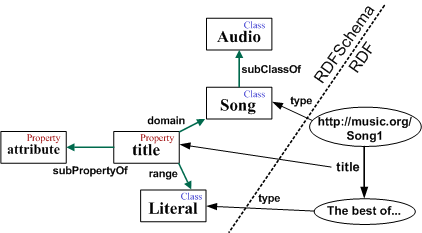
\includegraphics[height=2.5in]{images/RDFSchema.png}
	\caption{RDF Schema sample}
\label{fig:images_rdfs_sample}
\end{figure}

RDFS is described in RDF style using: \\
- core classes like: \\
  - `rdfs:Resource' (all objects/resources) \\
  - `rdfs:Class' (all classes) \\
  - `rdfs:Literal' (all literals) \\
  - `rdfs:Property' (all properties) \\
  - `rdfs:Statement' (all reified statements) \\
- core properties like: \\
  - `rdfs:type' (specify kind of class) \\
  - `rdfs:subClassOf' (specify inheritance between classes) \\
  - `rdfs:subPropertyOf' (specify inheritance between properties) \\
  - `rdfs:domain' (specify domain restrictions) \\
  - `rdfs:range' (specify range restrictions) \\
- container classes like: \\
  - `rdf:Bag'  (unordered list of entitites) \\
  - `rdf:Seq'  (ordered list of entities) \\
  - `rdf:Alt'  (list of alternatives/choices) \\
  - `rdf:Container' (superclass for all containers) \\
- utility classes like: \\
  - `rdfs:seeAlso', `rdfs:isDefinedBy' (links and references to other entities) \\
  - `rdfs:Comment' (comments and notes of entities) \\
  - `rdfs:Label' (human-friendly name of entities) \\
\\

Missing features in RDFS: \ldots  \\
\\
Complex Ontologies in Web Ontology Language (OWL): \\
\ldots \\
\\

% section semantic_ontologies (end)

\subsection{Query Language}
\label{sec:semantic_querylang}

SPARQL requires a \textbf{triple store} - a database containing RDF documents \\
is also referred to as a \textit{Graph Store} \\
data is inserted via Bulk load operation or via SPARQL update statements \\
SPARQL consist of SPARQL Queries that are send over the SPARQL protocol \\
Clients sends the queries to an HTTP endpoint \\
Stores on the public Web incl. dbpedia.org, ckan.org, wikidata.org \\
SPARQL also works with RDFS \\
SPARQL has similarities to SQL:
- each element in a triple might be replaced with a variable like `?varName' like so: \\
\texttt{sample.sparql:}
\begin{lstlisting}[basicstyle=\ttfamily,numbers=left,numberstyle=\footnotesize\ttfamily,backgroundcolor=\color{sourcegray}]
  PREFIX ns1:<URI>
  PREFIX ns2:<URI>
  PREFIX ns3:<URI>

  SELECT ?varName
  WHERE {
      ns1:subject ns2:predicate ?varName
  }
\end{lstlisting}
- in the WHERE clause it hosts the graph pattern to match (could be cascaded to go down subgraphs) \\
- variables can occur at any place in the graph pattern (?subj ?pred ?obj) as select with query everything \\
\\
LIMIT \textless n\textgreater option at the end for limiting the result set \\
FILTER (?varName \textless condition\textgreater ) in graph pattern can restrict results to match some
literal values and supports: \\
- numbers, dates: \textless, \textgreater, = \\
- strings: =, regex() \\
\\
\textbf{open world} assumption: resources on the Web are described in different schematas with various properties
using different vocabularies \\
- UNION option in graph pattern combines different matches \\
- OPTIONAL option in graph pattern only returns those entities if they are available (otherwise empty) \\
\\
ASK query checks for the existence of a given graph pattern \\
CONSTRUCT can be used to retrieve a subgraph from a larger graph, can also be used to translate between different schemas \\
\texttt{sample2.sparql:}
\begin{lstlisting}[basicstyle=\ttfamily,numbers=left,numberstyle=\footnotesize\ttfamily,backgroundcolor=\color{sourcegray}]
  PREFIX ns1:<URI>
  PREFIX ns2:<URI>
  PREFIX ns3:<URI>

  CONSTRUCT {
      ?varA ns2:predicate ?varB .
      ?varA ns3:predicate ?literalA .
  }
  WHERE {
      ?varA ns1:predicate ?varB
  }
  FILTER ( ?varB > x )
\end{lstlisting}

% section semantic_querylang (end)

\subsection{Agents and Rules}
\label{sec:semantic_logic_rules}


% section semantic_logic_rules (end)

% section semantic_web (end)
